\section{Representation-Based Compression: MRCZ}\label{sec:mrcz}

This section presents MRCZ, a representation-based compressor with a strict pointwise error guarantee. Section~\ref{sec:mrcz:overview} provides an overview of its compression workflow and explains how residual quantization enforces the user-specified error bound. Section~\ref{sec:mrcz:transform} examines the selection of the transform and coefficient error bound, including why MRCZ applies DChT rather than the conventional DLT to data sampled on GLL nodes. Section~\ref{sec:mrcz:transpose} reorganizes the quantized transform coefficients to improve their regularity and the effectiveness of lossless encoding.

\subsection{Overview of MRCZ}\label{sec:mrcz:overview}

Before presenting the MRCZ workflow, we briefly revisit the transform-based compressor of Marin et al.~\cite{marin2016spectral}. During compression, it applies a basis-matched transform to each element, discards information by setting selected coefficients to zero, and encodes the resulting coefficient stream. Inverse-transforming this lossy representation during decompression therefore generally does not reproduce the original data exactly. Moreover, the compressor provides no mechanism for enforcing a pointwise error bound.

\begin{figure}[htb]
    \centering
    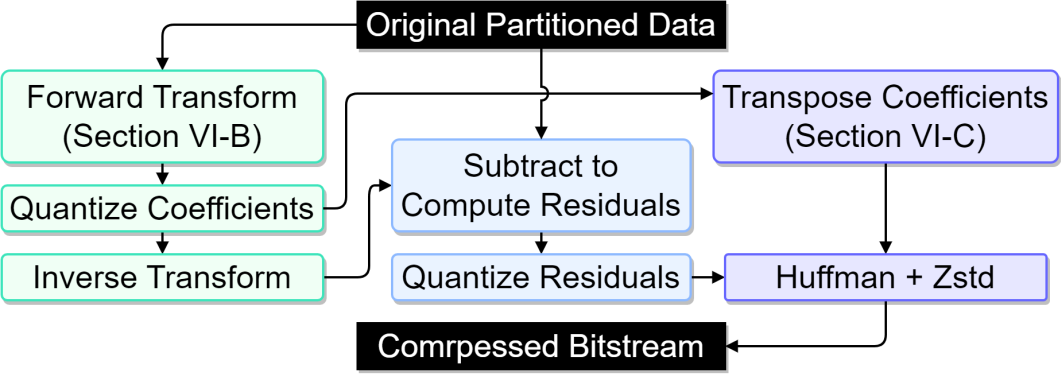
\includegraphics[width=1\linewidth]{figs/6/mrcz diagram.png}
    \caption{Overview of the MRCZ compression workflow.}
    \label{fig:mrcz_diagram}
\end{figure}

As illustrated in Figure~\ref{fig:mrcz_diagram}, MRCZ likewise represents each element in transform coefficient space, but treats the inverse transform of the quantized coefficients as a prediction rather than the final reconstruction. During compression, MRCZ computes the residual between this prediction and the original data and quantizes it under the user-specified error bound. During decompression, the same prediction is reproduced and corrected using the reconstructed residual. The final reconstruction error therefore equals the residual quantization error, providing a strict pointwise guarantee. Because this guarantee is enforced through residual quantization, the transform coefficients can be quantized under a separate internal error bound $\varepsilon_{\mathrm{coeff}}$ that need not equal the user-specified absolute error bound.

Finally, MRCZ forms its bitstream from two symbol streams: transform coefficients quantized under the internal coefficient error bound and prediction residuals quantized under the user-specified absolute error bound. Both streams are losslessly encoded using Huffman coding followed by Zstandard. Before encoding, MRCZ reorganizes the coefficient stream from element-major to mode-major order to improve its compressibility, as discussed in Section~\ref{sec:mrcz:transpose}.

\subsection{DChT for Data on GLL Nodes}\label{sec:mrcz:transform}

DLT is conventionally paired with data sampled on GLL nodes because the GLL nodes and their associated quadrature weights preserve the weighted orthogonality of distinct Legendre modes~\cite{marin2016spectral}. MRCZ, however, independently enforces the final reconstruction bound through residual correction, so its transform needs only to be invertible and numerically stable. It need not be orthogonal under the GLL quadrature weights. This freedom allows MRCZ to select the transform according to the compressibility of its coefficients and residuals. We therefore examine whether another commonly used transform can yield better compression than DLT for data sampled on GLL nodes.

We compare DLT, DCT, DST, and DChT under two coordinate assumptions. The ``GLL'' variants construct the transform matrices using the actual GLL coordinates, whereas the ``Uniform'' variants treat the same values as samples at uniformly spaced coordinates. For each evaluated combination, we vary the internal coefficient error bound introduced in Section~\ref{sec:mrcz:overview}, since it changes prediction accuracy and hence compression. We parameterize this bound as $\varepsilon_{\mathrm{coeff}}=\alpha\varepsilon_{\mathrm{abs}}$, where $\alpha$ is the coefficient-bound ratio. The best $\alpha$ may differ across transforms. Decreasing $\alpha$ improves prediction and lowers the residual BR but raises the coefficient BR. If too small, both the coefficients and predicted values are more accurate than needed to satisfy the user-specified bound. Increasing $\alpha$ reverses this tradeoff, lowering the coefficient BR but raising the residual BR and reducing PSNR as prediction worsens. The user-specified bound always sets a lower bound on the final PSNR.

\begin{figure}[htb]
    \centering
    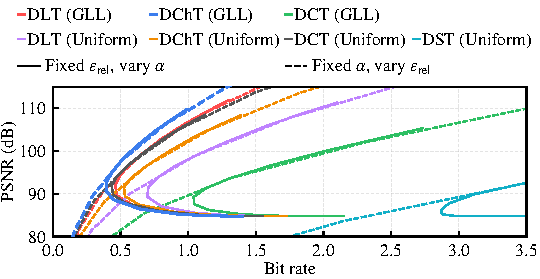
\includegraphics[width=\linewidth]{figs/6/transform-comparison-stacked.pdf}
    \caption{Rate--distortion performance of the transform--coordinate combinations. DChT evaluated at the GLL coordinates achieves the best overall performance, improving the compression ratio over DLT at the same coordinates by 17.5\% on average at matched PSNRs.}
    \label{fig:transform}
\end{figure}

Figure~\ref{fig:transform} compares the rate--distortion behavior of the evaluated transform--coordinate combinations. For each combination, it overlays the fixed-bound $\alpha$-sweep with the conventional rate--distortion curve obtained using the selected $\alpha$. The DST (GLL) combination is not shown because its transform matrix is singular. DChT evaluated at the actual GLL coordinates generally achieves the best rate--distortion performance. At matched PSNRs, it improves the compression ratio by 17.5\% on average over DLT evaluated at the same coordinates. We therefore adopt this configuration with $\alpha=0.05$ in MRCZ.

\begin{figure}[htb]
    \centering
    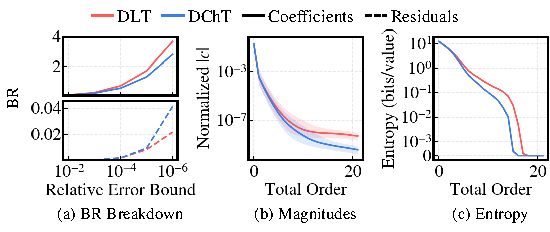
\includegraphics[width=1\linewidth]{figs/6/transform-mode-statistics.pdf}
    \caption{Comparison of DLT and DChT at the GLL coordinates on the $P$ field of Dataset~4. (a) DChT's smaller coefficient stream accounts for its compression advantage. (b)--(c) DChT produces smaller high-order coefficients and lower entropy of the quantized coefficients. Shading in (b) indicates the interquartile range.}
    \label{fig:transform-mode-statistics}
\end{figure}

Figure~\ref{fig:transform-mode-statistics}(a) compares the independently compressed coefficient and residual streams of DLT and DChT, both evaluated at the actual GLL coordinates. Across the five error bounds, the DLT coefficient BR is 1.25$\times$ that of DChT on average. In contrast, the ratio between the residual BRs is unstable, with DLT ranging from 0.52$\times$ to 1.37$\times$ that of DChT. Despite this relative variation, the coefficient BR is 67.7--2002$\times$ the residual BR and therefore dominates the compressed representation. The rate--distortion advantage of DChT thus comes primarily from its smaller coefficient stream.

Figures~\ref{fig:transform-mode-statistics}(b) and~\ref{fig:transform-mode-statistics}(c) explain this difference by grouping coefficients by total mode order. DLT and DChT are similar at low orders, but DChT produces progressively smaller coefficients at higher orders. At total order~15, the highest order at which both transforms retain nonzero entropy, the median DChT coefficient magnitude is 8.5 times smaller than that of DLT, while the entropy decreases from 0.031 to 0.00032 bits per coefficient.

\subsection{Improving Local Regularity for Lossless Encoding}\label{sec:mrcz:transpose}

We further investigate whether the quantized transform coefficients can be made more compressible by improving their local regularity before lossless encoding. A related idea is used in QoZ2.0~\cite{liu2024high}, which applies lightweight spatial blocking based on the observation that neighboring data points often exhibit similar prediction errors. Such regularity may arise because higher-order information not fully captured by interpolation can still exhibit local spatial continuity. Grouping quantized prediction errors within small spatial blocks therefore creates more regular symbol sequences and improves the effectiveness of subsequent lossless encoding.

However, the source of regularity in MRCZ differs from that in interpolation-based compressors. Neighboring entries in an element's coefficient matrix represent different basis modes and have no direct notion of spatial proximity. MRCZ therefore exploits regularity across elements by grouping coefficients associated with the same basis mode. This effect is particularly pronounced for higher-order modes, whose coefficients are frequently quantized to zero across many elements.

Motivated by these observations, we transpose the coefficient layout from element-major order to mode-major order, grouping coefficients associated with the same basis mode across multiple elements. This layout places frequently zero-valued higher-order coefficients and statistically similar same-mode coefficients into more regular sequences, improving the effectiveness of lossless encoding and increasing the compression ratio by approximately 20\%.
